\chapter{\label{chap:Novat} Le Style Novat}


\section{Contexte}


Parmi les panoramistes reconnus, Pierre Novat est l'artiste qui a dessiné et peint la plupart des panoramas des domaines skiables de France. Il travaillait avec des commanditaires locaux pour produire des panoramas de montagne servant de support aux plans des pistes du domaine skiable. Son travail était avant tout destiné aux habitants locaux et aux skieurs et était régi par des contraintes de politiques locales.

Aujourd'hui décédé, c'est son fils, Arthur Novat, qui a repris l'atelier et le travail de son père.  Pour empêcher que cette disparition entraîne une perte du savoir-faire de l'atelier, Arthur Novat essaye de transmettre son savoir et ses techniques à des chercheurs pour que celle-ci perdurent. 

Ainsi pour préserver la mémoire et la compréhension du travail de Pierre Novat, en 2015 débute le projet "MÉmoire, COnnaissance et MOdélisation de la Montagne : innovations et transfert d'outils de conception de plans panoramiques" (MECOMO) \footnote{MECOMO : \url{http://www.labexitem.fr/projet/memoire-connaissance-et-modelisation-de-la-montagne-innovations-et-transfert-doutils-de}}. C'est une collaboration entre géographes cogniticiens (INRIA), historiens (LARHRA) et informaticiens (LIG), autour de la conception de plans de pistes de ski par l'atelier Novat depuis la fin des années 1960. L’objectif global vise à reconstituer le fonctionnement de cette représentation dans le temps et donc dans l’évolution d’un système (les stations de ski), de manière à mieux comprendre le processus d’adéquation entre besoins, usages et représentation de l’espace au fil des années.
Cela s'articule autour de 3 axes : 
\begin{enumerate}
\item Historique: l’évolution des domaines skiables dans les Alpes et de ce qui les entoure. 
\item Cognition: la création et la lecture des panoramas de l'atelier Novat.
\item Informatique: l'automatisation de la création de panoramas.
\end{enumerate}

Ce projet a pris fin en 2017. Entre temps, plusieurs études ont été publiées notamment sur la création mental puis artistique d'un panorama fait par l'atelier Novat \cite{balzarini2015study} et sur l'analyse de la lecture des panoramas style Novat par les usagers \cite{balzarini2016effectiveness}. De plus un logiciel prototype a été créé au LIG pour permettre à un utilisateur de déformer des montagnes.  
Cependant, il reste encore beaucoup de recherche à faire pour pouvoir produire automatiquement des panoramas "à la Novat". 

En nous appuyant sur les études du projet MECOMO et en travaillant avec Arthur Novat, notre objectif est ainsi d'expliciter des règles de dessin et de les mettre en œuvre dans une application informatique. 
La production d'un logiciel prototype pour la création de panoramas permettra d'aider à la formalisation des règles et de les valider.

\section{Les panoramas de montagnes en informatique graphique}

Il y a deux travaux scientifiques qui ont été faits sur le rendu complet de panoramas de montagnes en informatique graphique. 

Le premier a été fait par Bratkova et al. en 2009 \cite{bratkova2009artistic}. Dans leur papier ils analysent les œuvres de Berann et James Niehus, deux artistes spécialisés dans les panoramas, et proposent un ensemble de principes pour le rendu de panoramas. Leur algorithme inclut des méthodes pour la déformation de terrain, la génération d'ombrage et de texture. Leurs résultats correspondent aux styles de Berann et James Niehus, toutefois leur méthode ne permet pas un rendu temps réel. 

Le second, fait par Brown et al. en 2017 \cite{brown2017real}, s'appuie sur les résultats du premier. Il présente une méthode pour un panorama interactif temps réel d'une région donnée. Comme pour le premier, leur algorithme inclut des méthodes sur la déformation de terrain, le rendu des couleurs (ombrage), le rendu des arbres, de l'eau et de l'atmosphère. Cependant, ces deux études n'explorent qu'en surface les différents éléments qui composent un panorama et produisent des résultats ressemblant mais loin d'être parfaits et qui comportent beaucoup de défauts. 

Nous allons suivre la même méthodologie que ces travaux : étudier le style de Pierre Novat pour en produire des règles de dessin et ensuite les appliquer dans un rendu 3D.



\section{Étude du style de Pierre Novat}

Pour cette étude, nous nous basons sur le livre : le plan des pistes, les domaines skiables de France dessinés par Pierre Novat \cite{novat2013plans} qui contient ses panoramas accompagnés de notes écrites par Frédérique Novat, Arthur Novat et Laurent Belluard, ainsi que sur les différentes interviews que nous avons pu faire avec Arthur Novat. Cependant cela reste des panoramas fait à la main et donc même si les règles citées ci-dessous sont généralement respectées, il existe toujours des contre-exemples.



\subsection{Qu'est-ce que dessiner un panorama du point de vue d'Arthur Novat ?}
Un panorama répond à la demande d’un commanditaire qui veut donner à voir une montagne de façon à la mettre en valeur. Cette demande porte en elle une part de fausseté car la représentation recherchée ne correspondra jamais à un point de vue réel. C’est une représentation d’un territoire imaginaire dans le but de le décrire au mieux et de le faire aimer. 
Le commanditaire est généralement un acteur important de la région : station de ski, collectivité locale, comité d'organisation des Jeux olympiques d'hiver, etc.

Le panorama des pistes de ski doit donc suivre certaines contraintes pour satisfaire le commanditaire mais aussi le skieur. Tout d'abord, les conditions météo et de luminosité doivent être optimales: avoir un ciel dégagé et un soleil matinal plutôt rasant révélant l'ensemble du relief. Ensuite, le panorama doit être équilibré géographiquement, c'est-à-dire que les étages alpins doivent être respectés : un point qui est en plus haute altitude qu'un autre, doit l'être sur le panorama. Même principe pour les dénivelés: plus une pente est inclinée, plus elle doit l'être sur le panorama. Enfin, au-delà des aspects purement géographiques les panoramas doivent aussi obéir à des contraintes sociales et politiques, c'est-à-dire qu'il faut respecter la concurrence entre les commendataires et la vision de la population locale. En effet, les villages présents sur le panorama veulent avoir une taille proportionnelle à leur investissement dans la station. Mais il faut aussi que la population locale puissent reconnaître sa région dans le panorama en ayant un point de vue reconnaissable ou des éléments marquants du paysage mis en avant. Par exemple Chamrousse est une station de ski visible depuis Grenoble et utilisée principalement par ses habitants donc le panorama a comme point de vue celui de Grenoble. 
D'un autre coté, les lieux importants doivent être mis en valeur et au contraire les lieux moins accessibles doivent être amenuisés. Enfin, les pistes doivent avoir une bonne représentation: elles doivent toujours descendre, les types de pistes (verte, bleue, rouge ou noire) doivent être vues de la même façon (même si en réalité les pistes vertes sont plus courtes que les noires), et le lecteur doit pouvoir différencier les pistes noires des pistes vertes uniquement grâce à leur forme (sinueuse pour les vertes, droite pour les noires).


\subsection{Fabrication en pratique - Les différentes étapes}

\begin{figure*}[h!]
\centering
 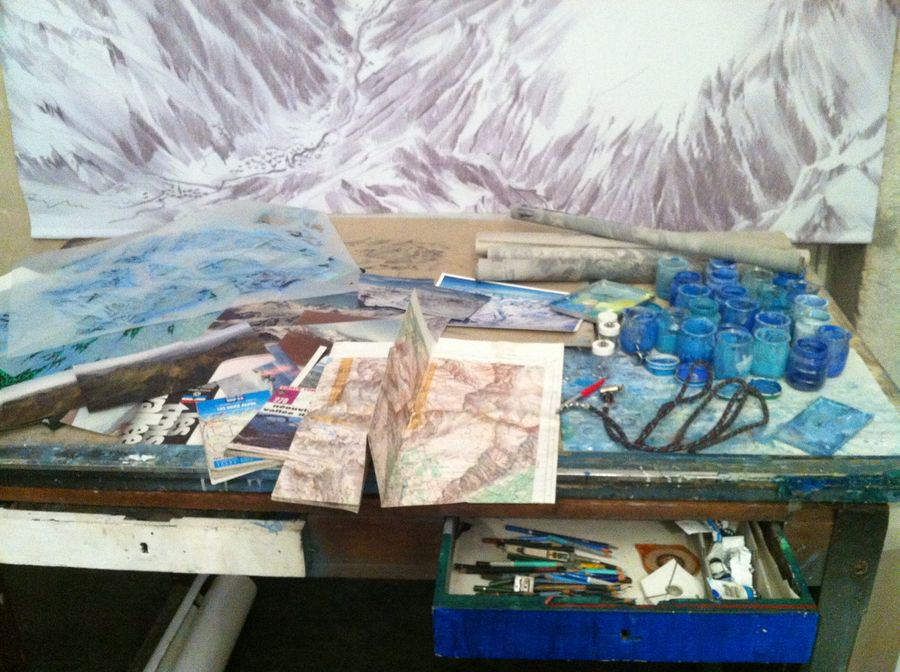
\includegraphics[width=0.5\linewidth]{novat/PN_Modelisation.jpg}
 \caption{\label{fig:Model} Pêle-mêle de photos et de cartes}
\end{figure*}


Maintenant que nous avons vu les règles générales des panoramas style "Novat", nous nous penchons sur la fabrication concrète d'un panorama. Pour faire des panoramas Pierre Novat utilisait, en fonction des territoires et de son inspiration, de la gouache, un aérographe, des feutres et des crayons de couleur; le tout appliqué sur une couche d'acrylique Gesso. Il y avait aussi un cheminement précis pour la création d'un panorama mis en place par l'atelier Novat : 
\begin{enumerate}
%\baselineskip=10pt
\item Le point de départ est une carte d'état major, de l'Institut national de l'information géographique et forestière (IGN) TOP25 ou autre. Elle sert à comprendre le terrain (Arthur Novat interprète les courbes de niveau comme un volume) et à choisir le point de vue.
\item Une collecte d'information s'ensuit : étude de la nature du terrain, photos (au sol, en avion, satellite) et visite sur place. Le but est de comprendre la physionomie du paysage. 
\item Prise en compte de la demande du commanditaire en dépliant le paysage. Construction d'un pêle-mêle de photos et de cartes. (Fig. \ref{fig:Model})
\item Création d'un crayonné à partir du pêle-mêle (calque et crayon ou photoshop). Un crayonné est un dessin en niveau de gris qui correspond principalement à l'ombrage mais il contient aussi toutes les éléments nécessaires au panorama (Fig. \ref{fig:crayonne}).
\item Validation par le commanditaire.
\item Mise en couleur :
\begin{enumerate}
\item Décalquage du crayonné au crayon de couleur (colorier au crayon de couleur sur un calque, le retourner sur le support et tracer l'esquisse).
\item Ajout de soutiens : crayon de couleur pour soutenir les arêtes ou les zones saillantes. 
\item Application d'une couche d'aérographe à la gouache avec utilisation de rhodoïds pour masquer.
\end{enumerate}
\item Dessin des détails : (Fig. \ref{fig:courchevel})
\begin{itemize}
\baselineskip=10pt
\item Sapins au crayon de couleur;
\item Rochers en peinture et crayons;
\item Maisons en peinture et crayons;
\item Rehausse du blanc en peinture;
\item Gratter sur le gesso pour retrouver le blanc. 
\end{itemize}
\end{enumerate}



\begin{figure*}[h!]
\centering
 \begin{subfigure}[t]{0.47\textwidth}
 \centering
 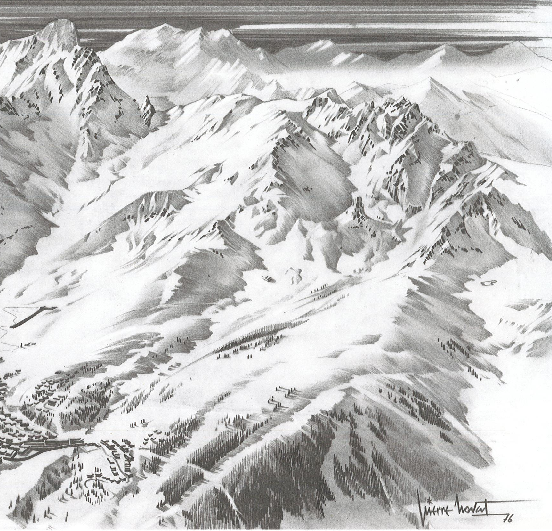
\includegraphics[width=1.0\linewidth]{novat/crayonn_.png}
 \caption{\label{fig:crayonne} Version crayonnée}
 \end{subfigure}%
 ~
 \hspace{.05\textwidth}
 \begin{subfigure}[t]{0.47\textwidth}
 \centering
 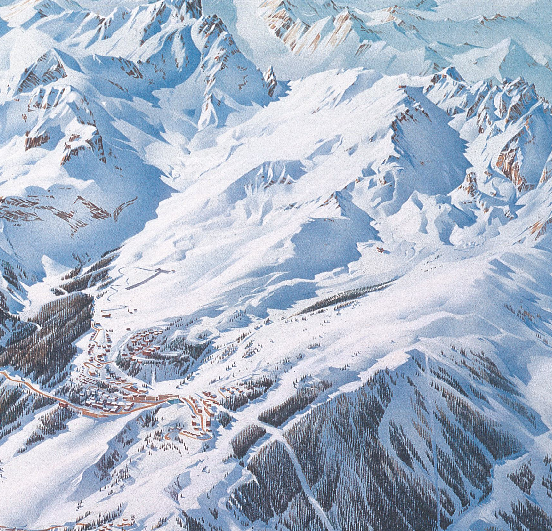
\includegraphics[width=1.0\linewidth]{novat/courchevel.png}
 \caption{\label{fig:courchevel} Version colorisée}
 \end{subfigure}
 \caption{Le panorama de Courchevel par Pierre Novat}
\end{figure*}



\subsection{Éléments visuels spécifiques du style Novat}
Intéressons-nous maintenant plus en détail à ces panoramas de style "Novat". Ils contiennent plusieurs éléments visuels qui n'ont pas la même importance. En effet si certains sont purement décoratifs, d'autres sont essentiels à la lecture et la compréhension du panorama. Nous décrivons ci-dessous les éléments visuels principaux par ordre d'importance.



\begin{figure*}[!h]
\centering
 \begin{subfigure}[t]{0.47\textwidth}
 \centering
 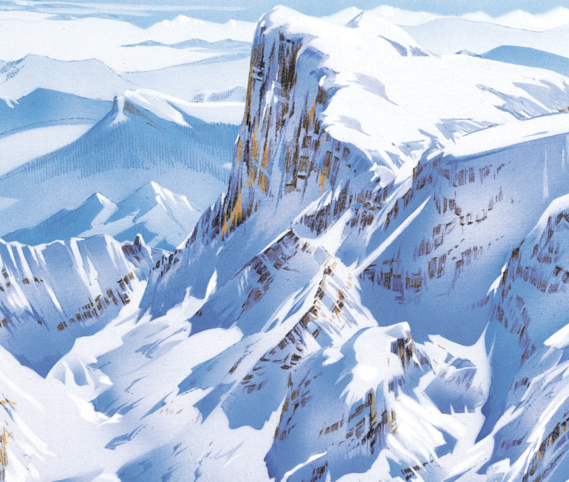
\includegraphics[width=1.0\linewidth]{novat/PN_zoom_ombre.png}
 \caption{\label{fig:zoom_ombre} Des ombres incohérentes mais lisible}
 \end{subfigure}%
 ~
 \hspace{.05\textwidth}
 \begin{subfigure}[t]{0.47\textwidth}
 \centering
 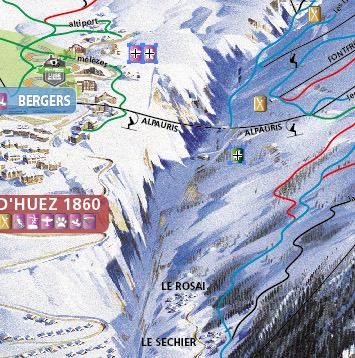
\includegraphics[width=1.0\linewidth]{novat/ombres_zoom.jpg}
 \caption{\label{fig:OmbrePortées} Ombres portées marquées sur le bord mais plus légères sur le flan de la montagne}
 \end{subfigure}
 \caption{\label{fig:ExOmbres} Exemples d'ombrage. %\ro{dans les 2 exemples, ce serait bien de mettre des flèches pour savoir exactement ou regarder (par ex: à quel endroit l'ombrage est différent d'un autre?)}
 }
\end{figure*}


\paragraph*{La lumière et les ombres :} 
Les variations d'intensité produites par l'illumination sont l'indice visuel principal pour comprendre la forme de la montagne. Elles peuvent ses séparer en deux composantes : ombrage et ombres portées. Ce sont toutes deux un signe d'une absence de lumière mais du à des causes différentes. Elles répondent à deux questions différentes : 
\begin{itemize}
\baselineskip=10pt
\item L'ombrage détermine si la surface est face à la lumière ou non. 
\item Les ombres portées déterminent si un autre élément cache la lumière. 
\end{itemize}
De plus le jeu des ombres amène des contrastes forts et tranchés qui donnent toute la nervosité du style de Novat. Seulement cette lumière est très irréaliste. Bien qu'il y ait une direction générale de la lumière (qui vient d'en haut, à droite ou à gauche), si nous regardons plus en détail, nous constatons que celle-ci n'est pas constante et peut être parfois totalement incohérente. Ainsi elle va plus être dirigée par la pente et les éléments que l'artiste veut montrer que par le respect de la réalité (Fig. \ref{fig:zoom_ombre}).
Enfin les ombres portées ne sont pas en conflit avec l'ombrage. En effet, les ombres portées sont rajoutées comme une couche supplémentaire plus légère que l'ombrage pour souligner le relief global sans pour autant gêner l'ombrage.  Aussi il est important de noter que tout a une ombre, que ce soient les montagnes, les petites bosses, les arbres, les maisons ou les routes. Ces ombres vont être orientées selon la forme de l’élément et la pente sur laquelle il repose.



D'autre part, les ombres ne sont pas d'une couleur uniforme (Fig. \ref{fig:OmbrePortées}) . Cela vient de deux facteurs. Le premier est que la montagne peut réfléchir la lumière et donc la montagne qui lui fait face aura une tache lumineuse pour indiquer cette inter-réflexion. Le second vient de la méthode de dessin. Pour dessiner ces ombres Arthur Novat va mettre un coup de crayon ou de couleur le long de l'ombre (généralement en bas), puis il va aplatir et étirer ce trait en le faisant remonter le long de la pente. Enfin les ombres sont très anguleuses. 
Tout ce travail a pour but de rendre très claire la lecture de la montagne et de la comprendre.









\paragraph*{La neige :} C'est un élément assez important car elle permet de connaître la nature du terrain. Il y a 3 types de terrain qui se dégagent : les glaciers qui sont verts et assez lumineux, la neige sur pente molle qui est très claire et réfléchissante et enfin la neige sur pente dure qui est plus sombre et mate. De plus la neige a un dégradé de couleur entre la haute altitude et la basse altitude. En haute altitude, la neige est proche du vert à cause des glaciers. En basse altitude par contre la neige sera plus bleue du fait de l’atmosphère.  


\paragraph*{Les arbres :} Leur importance vient de leur organisation. Le but de cette organisation est d'améliorer la perception de la forme de la montagne en plus des ombres. Pour ce faire, ils sont alignés verticalement et dans le sens de la pente. De plus il peut y avoir un trait sombre sur le bas des forêts pour marquer les ruptures de pente. 
Les arbres sont de couleur verte, allant du vert très foncé presque noir à l'ombre au marron-vert et quelque fois vert très clair en lumière. Il existe aussi quelques sapins blancs. Enfin ils sont toujours dessinés de manière verticale. Au $1^{er}$ plan, ils ont une forme légèrement triangulaire, au fond ils sont ovales, très fins et pointus au bout.  




\begin{figure*}[h!]
\centering
 \begin{subfigure}[t]{0.47\textwidth}
 \centering
 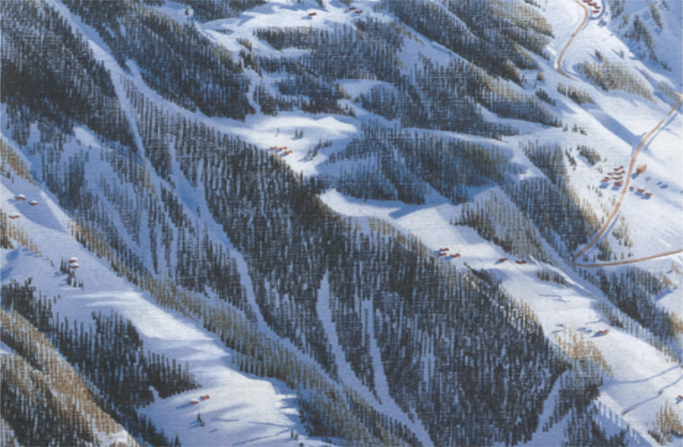
\includegraphics[width=1.0\linewidth]{novat/arbres_zoom.png}
 \caption{\label{fig:foret} Une foret sur un flan de montagne}
 \end{subfigure}%
 ~
 \hspace{.05\textwidth}
 \begin{subfigure}[t]{0.47\textwidth}
 \centering
 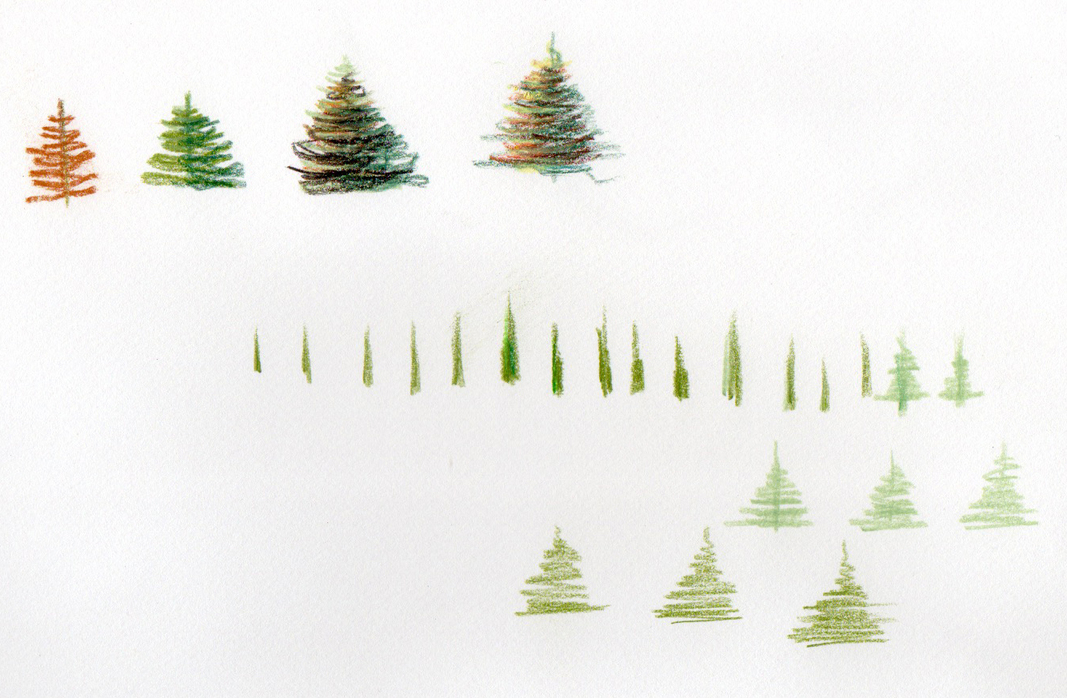
\includegraphics[width=1.0\linewidth]{novat/novat_arbre.jpeg}
 \caption{\label{fig:sapinseuls} Sapins dessinés par Arthur Novat}
 \end{subfigure}
 \caption{\label{fig:ExArbres} Exemples d'arbres}
\end{figure*}


\paragraph*{Les roches :} Elles sont moins importantes que les autres éléments cités plus haut mais elles ont quand même deux utilités. Elles sont soit informatives : elle servent à indiquer les barres rocheuse ou les pentes très raides où la neige ne peut pas tenir, donc des zones dangereuses; soit décoratives et servent de point de repère pour des zones rocheuses très identifiables de la région. Ainsi les roches sont organisées le plus souvent en lignes horizontales qui peuvent faire penser à des strates. Mais ces lignes ne sont pas continues, il y a toujours de fines bandes de neige qui passent entre les rochers et les délimitent. Enfin, elles se situent la plupart du temps juste en dessous des sommets des montagnes (Fig. \ref{fig:falaise}).

La couleur des rochers est unie. Elle va du gris clair, marron clair en lumière au marron foncé, noir à l'ombre. Leur forme est rectangulaire mais suit la forme de la montagne. La taille d'une roche varie selon la forme de la montagne (Fig.\ref{fig:rochersseul}).



\begin{figure*}[h!]
\centering
 \begin{subfigure}[t]{0.47\textwidth}
 \centering
 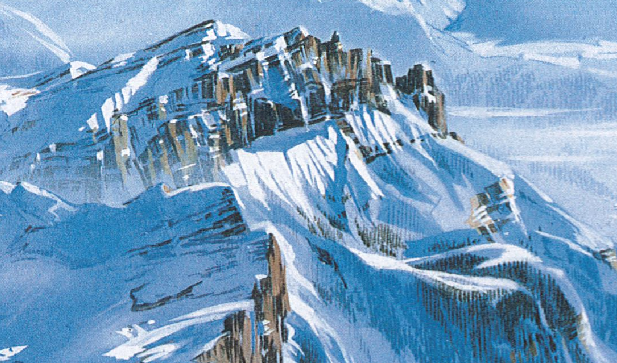
\includegraphics[width=1.0\linewidth]{novat/rochers_zoom.png}
 \caption{\label{fig:falaise} Une falaise}
 \end{subfigure}%
 ~
 \hspace{.05\textwidth}
 \begin{subfigure}[t]{0.47\textwidth}
 \centering
 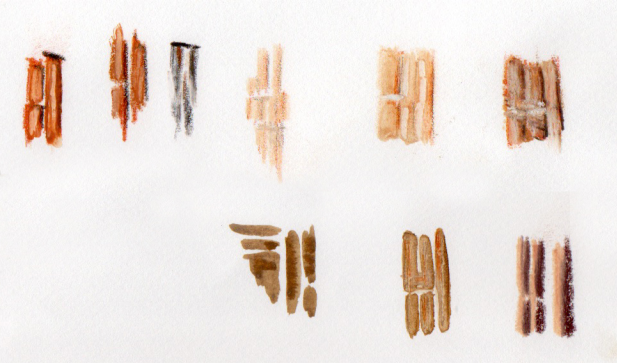
\includegraphics[width=1.0\linewidth]{novat/novat_roches.png}
 \caption{\label{fig:rochersseul} Roches faites par Arthur Novat}
 \end{subfigure}
 \caption{\label{fig:ExRoche} Exemples de roches}
\end{figure*}

\paragraph*{Les Maisons :} Purement décoratives, les maisons représentent les villes et villages de la région. Marron avec un toit blanc, leurs formes sont minimalistes mais correspondent à la réalité. Leur utilité est de servir de point de repère (Fig. \ref{fig:ExMaison}).


\begin{figure*}[h!]
\centering
 \begin{subfigure}[t]{0.47\textwidth}
 \centering
 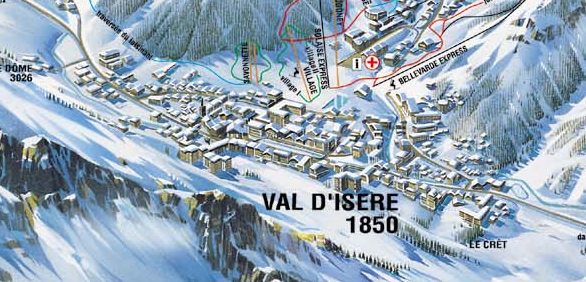
\includegraphics[width=1.0\linewidth]{novat/PN_maison.png}
 \caption{\label{fig:village} Le village de Val D’Isère}
 \end{subfigure}%
 ~
 \hspace{.05\textwidth}
 \begin{subfigure}[t]{0.47\textwidth}
 \centering
 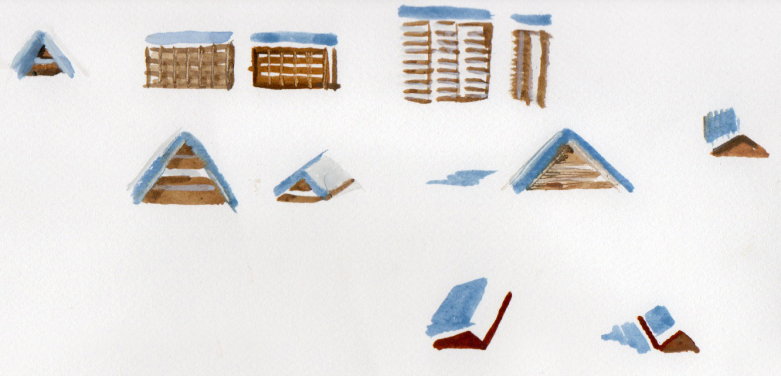
\includegraphics[width=1.0\linewidth]{novat/novat_maison.png}
 \caption{\label{fig:maisonsseul} Maisons faites par Arthur Novat}
 \end{subfigure}
 \caption{\label{fig:ExMaison} Exemples de maisons}
\end{figure*}

\paragraph*{Les routes :} Dessinées d'un trait continu, elles suivent fidèlement les routes existantes. Elles forment un creux dans la neige là ou elles passent. 

\paragraph*{L’arrière plan :}
Il est constitué uniquement de montagnes dessinées beaucoup plus simplement et avec bien moins de détails. Néanmoins, ces montagnes reste identifiables et reconnaissables pour quelqu'un qui connaît la région (Fig. \ref{fig:ciel}). 

\paragraph*{Le ciel :} Il est dégradé de bleu, avec quelques nuages. D'un bleu assez clair en bas, il fini très sombre en haut du panorama.   

\begin{figure*}[!t]
\centering
 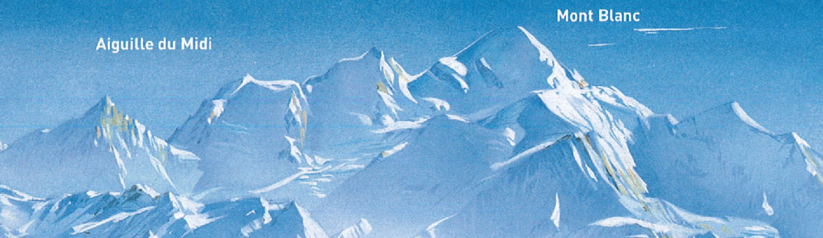
\includegraphics[width=1.0\linewidth]{novat/ciel_zoom.png}
 \caption{\label{fig:ciel}L'arriere plan du panorama du Grand Massif avec l'aiguille du Midi et le Mont Blanc qui sont reconnaissable}
\end{figure*}
